% -*- root: ../../main.tex -*
%!TEX root = ../../main.tex
% vim:textwidth=80 fo=cqt

\graphicspath{{chapters/layer_opt/figures/}}
% ----------------------- contents from here ------------------------

\chapter{Model-based Design Of Pouch Cells}\label{ch:modelbaseddesign}
\vspace*{-1em}
\startcontents[chapters]
\printcontents[chapters]{}{1}{\setcounter{tocdepth}{1}}

\bigskip

\glsunset{xeV}

% A brief  1-2 sentences throwback to  the literature review, referring  what we
% will say in this chapter.

\section[Introduction]{Introduction\protect\footnote{\textbf{Attribution      of
        content}  \   The  groundwork   for  converting   the  existing   computer  code
        (LIONSIMBA~v1.0$x$) into a suitable form for layer optimisation was initiated by
        this  thesis  author,  \mbox{Krishnakumar  Gopalakrishnan}.  However,  with  the
        exception of  the spectral scheme, for  which \mbox{Krishnakumar Gopalakrishnan}
        was  responsible, and  the zero-dimensional  thermal model  for which  \mbox{Ian
        Campbell} was  responsible, the advancements  inherent to the  enhanced computer
        software  (LIONSIMBA~v2.0)  were  made  in  equal  parts  by  \mbox{Krishnakumar
        Gopalakrishnan} and \mbox{Ian Campbell}. These  advancements would not have been
        possible without the contributions and support of Dr.~Davide Raimondo who served
        as an unofficial  supervisor for the work reported in  this chapter. The concept
        of layer reconfiguration for energy  and power trade-off, the layer optimisation
        framework, and the  source code by which it is  implemented were co-developed in
        equal  parts  by  \mbox{Krishnakumar Gopalakrishnan}  and  \mbox{Ian  Campbell}.
        \mbox{Krishnakumar Gopalakrishnan} was the  major contributor to the development
        of the binary search while \mbox{Ian  Campbell} was the major contributor in the
        analysis of results. \mbox{Parvathy  Chittur Subramanianprasad} was instrumental
        in  developing the  analytical expression  for  the maximum  possible number  of
layers~$n_\text{max}$.}}

The issue of `range anxiety' is a pervasive mental blockade for potential buyers
of electric  vehicles which  in-turn hampers their  widespread adoption.  From a
consumer viewpoint, yet another practical issue is the fact that on encountering
a  `low  battery' scenario  in  a  long  distance  journey, the  charging  times
required for sufficiently  replenishing the battery to enable  completion of the
journey are prohibitively  large, to the point of  being non-competitive against
conventional fossil  fuel powered  vehicles.

Unfortunately,  the  aforementioned  scenarios  are not  unimaginable  with  the
present  state  of the  art  in  lithium  ion  batteries. Hence,  improving  the
\gls{aer} and  providing fast charging  capabilities are two near-term  goals of
manufacturers  of electric  vehicles.  Increasing the  \gls{aer} necessitates  a
battery pack with  higher energy content in it while  lowering the charging time
demands a  pack with higher  power capability.  The contrasting nature  of these
goals can  be traced  all the way  down to  the cell level  and is  presented in
\cref{sec:energypowertradeoff}. By trading  off the number of layers  in a pouch
cell  against  the content  of  active  electrode material  accommodated  within
it,  bespoke cell  designs  addressing either  the energy  demand  or the  power
demand  can  be  obtained.  In  the  absence  of  accessible  documentation  (as
either  industry white  papers or  academic literature)  on the  layer selection
methodologies employed in automotive pouch  cell designs, this author postulates
that manufacturers  iterate through  an extensive  empirical testing  process of
prototypes with  a range of  layer choices. In the  view of this  thesis author,
this  procedure is  not only  time-consuming, but  is also  likely to  result in
sub-optimal designs.  This chapter envisages a  model-based engineering solution
to more  optimal cell designs  by determining  the appropriate number  of layers
needed  to maximise  its  \emph{usable} energy  while simultaneously  satisfying
certain  power  capability constraints.  The  rest  of  the chapter  provides  a
detailed treatment of topics such  as the proposed layer optimisation framework,
its assumptions involved,  and various modifications to  standard numerical code
required to facilitate this design procedure.

\section{Energy/Power Trade-off in Pouch Cells by Layer Selection}\label{sec:energypowertradeoff}

Varying the  number of electrochemical  layers stacked  within a pouch  cell has
contrasting effects  on its energy  storage and power handling  capabilities. In
this section,  a high-level  intuitive explanation of  this phenomenon  is first
offered, before  delving into  a detailed  presentation of  this effect  and its
implications for a specific  example cell in \cref{sec:energypowertradeoffdemo}.
Interwoven into the  narrative is a set of simplifying  assumptions made by this
thesis  author, which  sets the  broader  context within  which a  computational
framework for  determining the optimum  number of  layers for a  specific target
design shall be formalised and presented in \cref{sec:layeroptframework}.

\subsection{Preliminary assumptions}\label{subsec:layeroptassumptions}

To  obtain a  balanced  loading of  both electrodes  and  to avoid  asymmetrical
exhaustion  of lithium  from  one  of the  electrodes  during  operation, it  is
desirable to carefully calculate the  volume of electrochemical active materials
to be accommodated  within the cell. This concept is  well-known and is commonly
discussed  in  standard  textbooks in  the  field  such  as  those by  Rahn  and
Wang~\cite{Rahn2013} wherein  example calculations are presented  for non-porous
electrodes.

In  the  case  of  lithium  ion   cells  with  porous  electrodes,  the  concept
of  electrode-balancing  involves an  additional  variable  \viz{} the  porosity
of  the  active materials.  The  role  of  porosity  and its  corollaries  \ie{}
the  material  volume  fraction  and  filler/binder  fraction  is  discussed  in
\cref{subsec:spmp2dparametrisation}.  In this  work,  a  major assumption  about
material porosities  (and hence active-material/filler volume  fraction) is that
they are held constant. The rationale behind using this simplified assumption is
as follows.

This  author  visualises  the  integration  of  cell-level  design  optimisation
(through  an optimal  layer  selection procedure)  into  the overall  drivetrain
design  by the  \emph{cell manufacturer}  before  a custom  design is  delivered
to  vehicle/system  integrators.   Cell  manufacturers,  especially  small-scale
manufacturers do not necessarily  synthesize each electrochemical component, but
instead may opt  to source certain raw-materials from  an upstream supply-chain.
From  a  manufacturing  viewpoint,  the  porosity  of  the  electrode  materials
is  governed  by  the  extent  of  calendaring  of  the  electrode  reel.  Using
pre-calendered electrode materials or sourcing  large volumes of electrode reels
with a fixed extent of calendaring can help to keep costs low. In the absence of
a concrete  insight into  the procuring process,  this represents  a preliminary
justification of the author's assumption about constant porosities.

From a technical  viewpoint, there exists another redeeming  argument to support
the constant  porosity assumption. Keeping material  porosities constant enables
to eliminate a  degree of freedom in the design  optimisation, thereby narrowing
the dimensionality of  the search space. To the best  of the author's knowledge,
there has not  yet been any published work tackling  layer optimisation of pouch
cells.  Building an  initial  infrastructure \viz{}  a computational  framework,
based upon this constant porosity approximation shall provide a solid foundation
to build upon and extend for such  real-life use-cases. The author views this as
a vanguard research  into cell engineering and therefore places  a high value in
obtaining ballpark  estimates of  an optimal layer  count, albeit  with constant
porosities. Nevertheless,  the influence of  varying the material  porosities on
the cell's  performance is to be  quantified. Therefore, prior to  adopting this
model-based  methodology  for production  yields  at  scale, a  fully-integrated
design optimisation process  with variable porosities have to  be accounted for.
In this work, the author restricts the study to constant porosity values, whilst
acknowledging  variable  porosity designs  as  an  important aspect  for  future
studies.

At  a  system level,  the  efficiency  of the  drivetrain  is  considered to  be
constant. The  drivetrain of  an electric  vehicle consists of  a whole  host of
electrical as well as mechanical  components such as power electronics, electric
motors and  transmission. The efficiencies  of each  of these components  have a
cascading effect  on the overall  drivetrain efficiency. The efficiency  of each
component  is strongly  dependent upon  the operating  point. For  instance, the
efficiency of  an electric  motor is  a function of  its torque-speed  curve. In
practice, it  is rarely easy  to decouple  these efficiencies during  the design
stage. The datasheet/ technical specification  of each component in the platform
is required  to make  a comprehensive  multi-physics design  optimisation study.
This is well beyond the scope of this work and requires access to various design
blueprints. Therefore,  a constant  efficiency value is  adopted for  this work.
However, the  proposed optimisation methodology  is a modular one  which implies
that it can be adapted \eg{} to  include a efficiency value dependent upon power
delivered  at the  wheels. However,  the biggest  redeeming aspect  is that  the
constant efficiency does  not influence in any way the  final layer choice. This
is because  the drivetrain efficiency  comes into play only  during acceleration
studies and shall be discussed in \cref{sec:resultslayeropt}.

From  a  pack  perspective,  the   primary  assumption  in  the  formulation  of
the   proposed  optimisation   methodology  is   that  the   pack  configuration
(series/parallel arrangement  of modules, number  of cells per module  and other
system-level specifications) are held constant throughout. This validity of this
assumption  is easily  justified since  the cell-level  design may  be performed
independently of  the larger drivetrain  design. In fact, the  author postulates
that  present design  process for  electrified transportation  is a  modular one
\ie{} empirical cell designs are  developed based on certain specifications laid
out by vehicle  manufacturers and is not integrated into  the drivetrain design.
This  modularity  in the  design  approach  enables  to keep  such  system-level
parameters constant.

A further assumption  in this study is  that the overall height of  the pouch is
held constant. In  the absence of this constraint, any  arbitrary pouch size can
be chosen,  leading to an  infinite-dimensional optimisation problem  wherein no
definite optimality criterion  exists. This assumption is in-fact  enforced by a
current  trend  in the  automotive  industry  \viz{} adoption  of  common-module
designs wherein  the physical  dimensions of  the pack  are chosen  a~priori and
modularisation of pack helps in tailoring  of packs to cater to different market
segments.  Extending this  philosophy down  to  the cell  level, it  is easy  to
visualise the  benefits of  having cells of  identical exterior  dimensions. For
instance, having a  common inventory helps a vehicle manufacturer  to keep costs
in  check  for  subsequent  design  of drivetrains  \eg{}  in  derivative  model
families. This  means that, for  any layer choice  to be tried,  the constituent
components of the cell is to be arranged and contained within the same pouch (of
fixed  exterior dimensions).  This naturally  leads to  the assumption  that the
thickness of  the pouch  material used shall  remain constant  throughout, which
in-turn implies that the overall height  of the electrochemical stack within the
pouch is constant. The detailed calculations of the stack height is presented in
\cref{sec:layeroptframework}.

The  current collectors  and the  separator  in each  electrochemical layer  are
assumed  to  have  uniform  thickness  irrespective  of  the  number  of  layers
used. Barring  minor manufacturing variability  and tolerances, this  is factual
information requiring  no further  justification. The  final assumption  from an
electrochemical point of view is that the relative thicknesses of each electrode
is held  constant to a  fixed ratio. This  warrants further explanation,  but is
ill-suited  for this  introductory discussion.  The details  of this  aspect are
discussed in  \cref{sec:layeroptframework}. Certain  assumptions are to  be made
about the  temperature distribution  within the  layers owing  to the  choice of
cooling arrangement.  This aspect  merits more  than a  cursory listing  in this
introductory section and hence is discussed in \cref{sec:layeroptframework}.

\subsection{Motivation}\label{subsec:layeroptmotivation}

This section aims to provide a  qualitative description of the effect of varying
the number of  layers within the cell  and presents the motivation  to embark on
this layer optimisation effort.

Given the  assumptions listed in \cref{subsec:layeroptassumptions},  it is clear
that  changing the  number  of layers  in  a pouch  of  fixed thickness  results
in  different  absolute  electrode  thicknesses.   This  in  turn,  affects  the
electrochemical-thermal behaviour  of the  cell. Having a  low number  of layers
means  that the  proportion of  energy-storing  materials within  the volume  is
higher, leading  to greater stored  energy. However,  all of this  stored energy
might not be available for utilisation due to the large time constants necessary
for lithium ions to diffuse through  thick domains. Power handling capability of
the cell suffers  since ion deficits at electrode surfaces  lead to the collapse
of its terminal voltage.

Prima  facie, based  on  the  above discussion,  although  it  appears that  the
absolute lowest possible  number of layers (\ie{} one layer)  is the best choice
for maximising  driving range, there  exist two  other goals that  conflict with
this design  intent. Firstly, there must  be a minimum electrode  active surface
area  to  handle the  power  demands,  and hence,  a  minimum  number of  layers
typically far  greater than one. Higher  power capability is achieved  by way of
larger electrode surface  area and higher electrical  and thermal conductivities
owing to the presence of more current collectors. Secondly, the acceptable limit
on  lifetime  degradation of  cells  places  an  upper  bound on  the  allowable
temperature rise during vehicle operation. Increasing the number of layers has a
two-fold mitigating effect on the  temperature-rise experienced by the cell. The
\emph{power  density} within  each  layer  is diminished  due  to the  increased
available  surface area,  leading to  reduced ohmic  heat generation  within the
cell. With  each layer requiring a  Al-Cu current-collector pair, the  number of
heat conduction  pathways increases  linearly with the  number of  layers. Thus,
increasing the number of layers has a beneficial effect on pack lifetime.

In summary,  for very low number  of layers, there exists  more active material,
leading  to a  high  energy  capacity. However,  the  reaction  surface area  is
diminished proportionately leading to lower power capability. Furthermore, owing
to  the presence  of very  thick electrodes,  current density  within the  solid
conductive  matrix shall  not be  homogeneous~\cite{Pals1995}, nullifying  a few
modelling assumption  of the standard \gls{dfn}  model. On the other  hand, very
high number of layers imply vanishingly thin electrodes and correspondingly less
active  material  accommodated within  the  cell,  thereby lowering  its  energy
capacity.

Therefore, there exists  a research question on what constitutes  the best layer
choice  that straddles  this  trade-off  with the  least  penalty  to the  power
capability  of  the  cell  whilst simultaneously  having  the  maximum  possible
capacity. This  saddle point determination needs  to be performed for  a curated
set of power input/output conditions to the cell. This niche problem has not yet
been tackled and motivates the need to perform a careful design study documented
in this chapter.

\subsection{Quantitative demonstration of energy/power trade-off}\label{sec:energypowertradeoffdemo}

The discussion in \cref{subsec:layeroptmotivation} has motivated the need for an
in-depth exploration  of the energy to  power trade-off expressed as  a function
of  the number  of  layers.  Before embarking  on  constructing  a framework  to
optimise the  layer choice by  formalising various constraints that  govern this
optimality, this section aims to bring out this relationship by applying a fixed
galvanostatic discharge to  an example cell. Additionally,  the critical concept
of \emph{usable} energy versus \emph{total} stored energy is also introduced.

A  \gls{lco}  cell  whose  physical  properties  and  simulation  parameters  is
drawn from  the combined  set of  data from  \cref{tbl:lcoSimParamslayeropt} and
\cref{tbl:lcoSimParamsSPMp2d}  is used  as the  example  cell. The  only set  of
values that overlap between these two tables are ---
\begin{enumerate*}[label=\itshape\alph*\upshape)]
    \item the cut-off voltages, and
    \item the number of nodes  used for numerical  discretisation of  the governing  \gls{pdae} equations.
\end{enumerate*}
For these conflicting quantities,  the values in \cref{tbl:lcoSimParamslayeropt}
prevail for all simulation studies  in this chapter. Furthermore, the individual
electrode thicknesses  from \cref{tbl:lcoSimParamsSPMp2d} is not  directly used,
but  instead  calculated  for  every  layer  choice  by  keeping  the  ratio  of
their  relative  thicknesses  constant.  This   aspect  shall  be  explained  in
\cref{sec:layeroptframework}.

\Cref{fig:fig_CC_discharge_curves} illustrates  the influence  of the  number of
layers  on the  energy and  power capability  of the  example cell.  Starting at
\SI{100}{\percent} \gls{soc},  a constant current discharge  of \SI{60}{\ampere}
is applied  to a \gls{dfn}  model of the cell  until reaching the  lower cut-off
voltage. For  each discharge  run, the  model is  reconfigured with  a different
layer choice. Five distinct layer choices  have been carefully conjured so as to
provide a clear illustration of the energy/power trade-off phenomenon.

\begin{figure}[!bp]
    \begin{minipage}[t]{\textwidth}
        \centering
        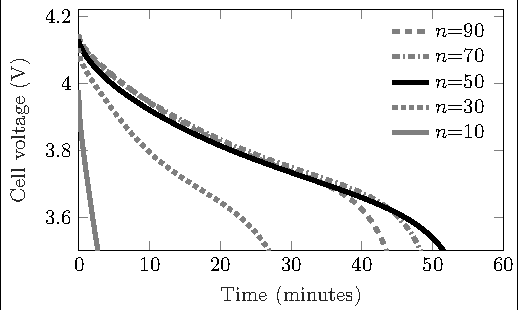
\includegraphics[trim=4 4 2 4,clip]{fig_CC_discharge_curves.pdf}
        \caption
        [%
        Voltage curves for a \SI{60}{\ampere} galvanostatic discharge from
        \SI{100}{\percent} \glsfmtshort{soc} until cut-off voltage for a few layer
        choices, in a pouch cell of fixed exterior height.
        ]%
        {%
            Terminal voltage curves of a Li-ion cell (with parameters
            given in \cref{tbl:lcoSimParamslayeropt}) under a \SI{60}{\ampere}
            galvanostatic discharge beginning from \SI{100}{\percent}
            \glsfmtshort{soc} until lower cut-off voltage for a few layer
            choices~$n$, in a pouch cell of fixed exterior height. The maximum
            usable energy is achieved for an intermediate choice of $n$
            that corresponds to neither the highest nominal capacity layer
            configuration ($n$=\num{10}) nor the highest electrode surface area
            configuration ($n$=\num{90})\footnotemark.
        }%
        \label{fig:fig_CC_discharge_curves}
        \mpfootnotes[1]
        \footnote{This figure was created by \mbox{Ian Campbell} who asserts copyright,
            with intellectual contributions from and the right to use asserted by
        \mbox{Krishnakumar Gopalakrishnan}.}
    \end{minipage}
\end{figure}

As  seen  in \cref{fig:fig_CC_discharge_curves},  during  the  initial phase  of
discharge, the terminal voltage  of the cell is the highest  for the two highest
layer choices  \ie{} $n  = 90$  and $n=70$. Consistent  with the  explanation in
\cref{subsec:layeroptmotivation}, these  two layer choices have  thin electrodes
and hence  comparatively low resistances  leading to only a  small overpotential
drop within the cell. However, as expected, their total energy is lower than the
cell with  $n=50$ layers as  evidenced by  their relative run-times  until lower
cut-off voltage.  This is to  be expected as the  thin electrodes of  these high
layer-count cells cannot  store a large volume of active  material. Based on the
explanation  from \cref{subsec:layeroptmotivation},  it  is  expected that  this
trend will  continue \ie{} the  lower the layer  count, the higher  the run-time
until cut-off. If this were the case, prima facie it seems that the optimisation
task is trivial.

Inspecting the discharge curves of lower layer choices brings into limelight the
concept of \emph{usable} energy. Contrary  to expectations, the discharge curves
corresponding  to very  low layer  counts in  \cref{fig:fig_CC_discharge_curves}
terminate even earlier than $n=50$. This is  owing to the fact that although the
total  stored energy  in cells  with low  layer counts  is much  higher, only  a
fraction  of it  is  usable.  This aspects  introduces  non-convex dynamics  (as
discussed below) to an otherwise linear optimisation task.

For  instance,  when $n  =  10$,  the terminal  voltage  of  the cell  collapses
instantaneously, reaching cut-off  voltage whilst its \gls{soc}  remains as high
as \SI{96}{\percent}. At very low layer  counts, the thickness of each electrode
is high. This presents a high resistance  to the flow of charges thereby leading
to  high overpotential  drops  within the  cell. The  usable  energy under  this
\SI{60}{\ampere} galvanostatic  discharge for various layer  choices is compared
in \cref{tbl:CC_discharge_curves_table}. It can be  seen that for very low layer
counts,  the usable  energy that  can be  extracted is  miniscule, albeit  their
theoretical  capacity~$Q_n$  are  in-fact  the highest.  The  usable  energy  in
\SI{}{\watthour} reported in \cref{tbl:CC_discharge_curves_table} is obtained by
multiplying the integral  of the area under each discharge  curve by the applied
current \ie{}  \SI{60}{\ampere} with  the appropriate  scaling of  the time-base
(from minutes to hours).

% -*- root: ../../main.tex -*-
%!TEX root = ../../main.tex

\begin{table}[!htbp]
    \caption
    [%
    Theoretical  capacity \&  usable energy  of a  Li-ion cell  for a  few layer
    choices under a \SI{60}{\ampere} galvanostatic discharge
    ]
    {%
        Theoretical capacity and usable energy of a Li-ion cell (with parameters
        given in \cref{tbl:lcoSimParamslayeropt}) for  a few layer choices under
        a \SI{60}{\ampere} galvanostatic discharge.
    }%
    \label{tbl:CC_discharge_curves_table}
    \centering
    \begin{tabular}{@{} S[table-format=2.0] S[table-format=1.2] S[table-format=2.2]  S[table-format=3.2] S[table-format=2.2] @{}}
        \toprule
        \multicolumn{1}{@{} l}{$n$} &  \multicolumn{1}{c}{\footnotesize C-rate} & \multicolumn{1}{c}{\footnotesize \makecell{Theoretical \\ Capacity  (\si{Ah})}} & \multicolumn{1}{c}{\footnotesize \makecell{Usable \\ Energy \si{(Wh)}}} & \multicolumn{1}{c @{}}{\footnotesize \makecell{Remaining \\ SOC  (\si{\percent})}} \\
        \midrule
        90 & 1.24 & 48.25 & 166.46 & 9.84  \\
        70 & 1.11 & 53.99 & 184.80 & 10.26 \\
        50 & 1.00 & 59.73 & 195.47 & 13.51 \\
        30 & 0.92 & 65.47 & 101.20 & 58.95 \\
        10 & 0.84 & 71.21 & 10.15  & 96.22 \\
        \bottomrule
    \end{tabular}
\end{table}


\Cref{tbl:CC_discharge_curves_table}  also brings  into view  the fact  that the
\mbox{C-rate} of the  cell becomes a variable quantity even  for a galvanostatic
discharge,  due to  the dependence  of  its nominal  capacity on  the number  of
layers~$n$.  This  represents  a  departure  from  the  norm  in  the  modelling
community, wherein the performance of cells  are quantified as a function of the
applied C-rate \eg{}  in \cref{ch:spmanalysis} and \cref{ch:newelectrolytemodel}
of this  thesis. However,  this preliminary  investigation has  quickly revealed
that this normalised  quantity does not hold much importance  in any study where
the number of layers within a pouch cell is varied.

Taking into account  these factors, a reasonable choice of  the number of layers
in  this specific  \SI{60}{\ampere} galvanostatic  application for  this example
cell  could  be $n=50$.  This  represents  a  practical compromise  between  the
surface area  available for  reaction and  the total  volume of  active material
accommodated.  This layer  selection offers  the highest  usable energy  for the
given discharge rate, out of the finite layer configurations considered.

In this  sample study, only  a handful of  layer choices were  considered, which
represents  only  a  small  possibility  of  the  overall  design  space  to  be
considered. Furthermore,  thermal considerations were  not explored so  far. For
robust  cell design,  manufacturers  shall need  a  widely applicable  model-led
design tool that  can tackle the wide-ranging possible scenarios  that can occur
in real-life operating conditions. A deterministic set of optimality criteria is
also to  be formulated. The choice  $n=50$, therefore does not  represent in any
way the general  optimal layer choice even for this  example cell. However, this
serves as an illustrative demonstration of the trade-offs in energy versus power
handling capability of a cell for  a specific set of conditions. Furthermore, it
introduces the  complicating aspect of  \emph{useable} capacity into  what would
have  otherwise been  a  trivial  exercise, thereby  setting  the  tone for  the
development of a general layer optimisation framework for pouch cells.

\section{Scope and Context within \glsfmtshort{xeV} Powertrain}

It is  important to provide the  contextual setting for this  layer optimisation
work since it is nestled deep  within the broader horizon of electric drivetrain
optimisation. \Cref{fig:fig_PowertrainSchematic}  provides a  graphical overview
depicting the hierarchical architecture of  a typical \gls{xeV} powertrain, from
the  system level  down to  a  single electrochemical  layer. The  rest of  this
section describes the scope of this  layer optimisation work and its integration
into this  overall architecture. A further  set of assumptions that  were deemed
inopportune to be discussed  in \cref{subsec:layeroptassumptions}, is introduced
at apropos junctures throughout this narrative.

\begin{figure}[!bp]
    \begin{minipage}[t]{\textwidth}
        \centering
        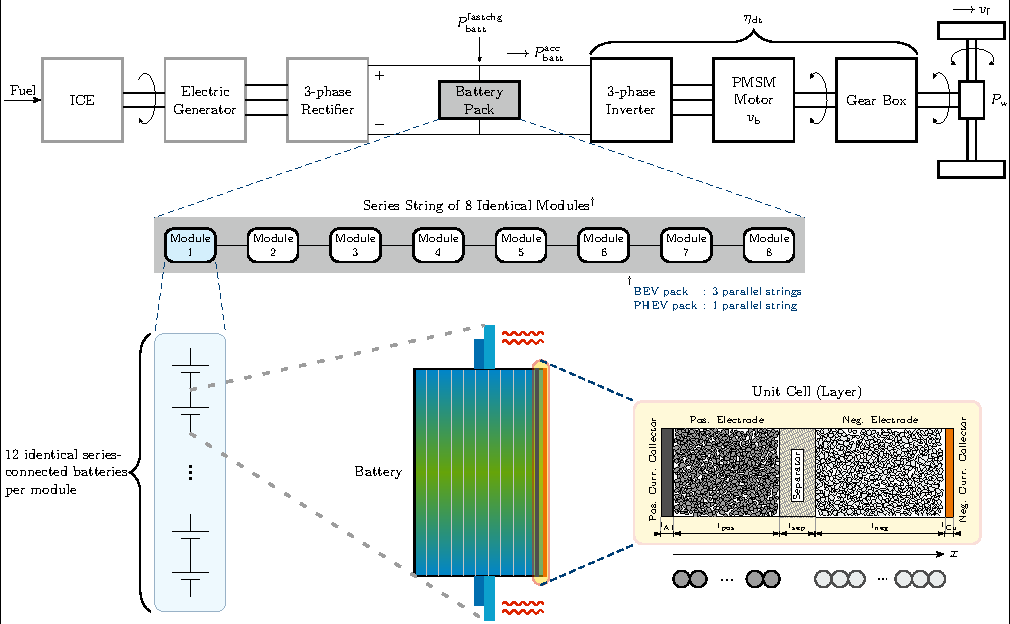
\includegraphics[width=\textwidth]{hierarchical_powertrain_to_cell_layer.pdf}
        \caption
        [%
        Vehicle-to-cell hierarchical overview of an electrified powertrain architecture.
        ]%
        {%
            Schematic depicting the vehicle-to-cell hierarchical overview of
            a typical electrified powertrain architecture. This represents the
            system-level context within which the proposed layer optimisation framework
            has been developed. Two \glsfmtshort{xeV} powertrains ---
            \begin{enumerate*}[label=\itshape\alph*\upshape)]
                \item a \gls{bev}, and
                \item a series \gls{phev}
            \end{enumerate*}
            are chosen as examples to demonstrate how the methodology facilitates
            common module designs for such battery packs\footnotemark.
        }%
        \label{fig:fig_PowertrainSchematic}
        \mpfootnotes[1]
        \footnote{This figure was created by \mbox{Krishnakumar Gopalakrishnan} who
            asserts copyright, with intellectual contributions from and the right to
        use asserted by \mbox{Ian Campbell}.}
    \end{minipage}
\end{figure}

\subsection{System-level architecture --- vehicular platforms}

The top row of  \cref{fig:fig_PowertrainSchematic} represents the typical layout
of a \emph{series}-hybrid powertrain~\cite{Emadi2017}. For partial supply of the
mechanical  power and/or  to  partially charge  the  battery during  propulsion,
a  downsized  \gls{ice}  coupled  to  the pack's  DC  bus  through  a  generator
and  three-phase  rectifier  is  employed. While  tackling  the  power  handling
requirements, irrespective  of whether a  \gls{bev} or \gls{phev}  powertrain is
being considered, the  cells in the pack  are to be designed  for the worst-case
operating  scenario,  \ie{}  without  any  power  support  from  the  \gls{ice}.
This  implies  that all  discharge  simulations  of  the  \gls{phev} are  to  be
conducted with the powertrain operating in  all-electric mode resulting in a net
charge-depletion. The only distinction is  that the \emph{magnitude} of power to
be handled by the  pack in this worst case scenario  is vastly different between
the  \gls{bev} and  \gls{phev} cases.  This allows  for some  simplification and
helps to narrow down the scope of the problem to be tackled as explained below.

Omitting the  components to the  left of the  battery pack (represented  as text
boxes with light grey border) shall render a powertrain corresponding to that of
a  \gls{bev}.  The proposed  layer  optimisation  methodology is  developed  and
presented in the context of this  \gls{bev} powertrain. However, being a modular
framework, the optimisation methodology may  be readily extended to a \gls{phev}
powertrain and shall be discussed in \cref{sec:commonmodulelayeropt}.

As  shown   in  \cref{fig:fig_PowertrainSchematic},  the   \gls{bev}  powertrain
typically comprises of ---
\begin{enumerate*}[label=\itshape\alph*\upshape)]
    \item a battery pack,
    \item a three phase inverter,
    \item a \gls{pmsm},
    \item a gearbox for  torque multiplication, and
    \item the rest of the  powertrain  (differential shaft  and driven  wheels).
\end{enumerate*}
Considering the  worst-case scenarios, the  power to  be handled by  the battery
pack arises due to  ---
\begin{enumerate*}[label=\roman*)]
    \item fast charging from  the mains~$P^\text{fastchg}_\text{batt}$ (charge), or
    \item acceleration  from standstill~$P^\text{acc}_\text{batt}$ (discharge).
\end{enumerate*}
The   acceleration  power   is  computed   from  the   power  required   at  the
wheels,  $P_\text{w}$  (the   details  of  this  calculation   is  presented  in
\cref{sec:layeroptframework}). The sign convention used  in this chapter is that
the  charging power  is positive  (and  consequently, the  discharging power  is
negative).

\subsection{Pack-level architecture --- strings, modules and cells}

Delving  into the  battery pack  under  consideration, this  thesis considers  a
standard  modular  layout wherein  the  \gls{phev}  pack  has one  string  while
the  \gls{bev}  pack  has  three  parallel strings.  Within  each  string,  both
vehicular platforms  employ 8~series-connected  modules. Taking  into cognizance
the  benefits  of common  module  design,  identical  pack modules  are  assumed
across  both  \gls{xeV}  platforms  which  is  then  extrapolated  to  impose  a
stronger  condition  of  identical  geometry  for  the  constituent  cells  (see
\cref{subsec:layeroptassumptions}). The exterior dimensions of the pouch cells
under consideration is listed in \cref{tbl:lcoSimParamslayeropt}.

Each module consists  of 12~series-connected identical cells  denoted by battery
circuit symbols (see cyan  filled blocks in \cref{fig:fig_PowertrainSchematic}).
The \gls{phev}  pack is smaller and  consists of \ordfrac{1}{3} of  the cells in
the \gls{bev} pack. Assuming that the \gls{bev} pack consists of a \mbox{96S-3P}
cell  assembly,  this implies  that  the  \gls{phev}  pack  shall conform  to  a
\mbox{96S-1P} layout. The DC~bus voltage is unaltered since both packs have same
amount of  series cells. The power  flow is assumed to  be uniformly distributed
across all  the cells within  the pack(s). At first,  the power required  at the
terminals of the  pack is computed. From this, a  first-order design ballparking
of the layers of the cell is made through a single cell simulation. This process
enables reduced simulation runtime with the conditions of one cell assumed to be
representative of all cells in the pack.


% At  a high-level,  the  essence of  the layer  optimisation  methodology can  be
% distilled down  to the following sequence.

While  this  assumption of  identical  cell  conditions  across the  pack  seems
infeasible  at first  glance, three  careful  considerations have  been made  to
justify  this assumption.  Firstly,  power  (and not  current)  is  used as  the
stimulus to the cell. This  implies that, despite the \emph{parallel} connection
of cells  (in groups of three  cells within each module),  each cell experiences
the same  power. Even  across parallel-connected strings,  the power  handled by
each cell shall be the same.  This necessitates the modification of the standard
\gls{dfn}  model in  order to  accommodate power  inputs which  is discussed  in
\cref{sec:innatepowerinput}. Secondly,  although the current  in all cells  of a
\emph{series}  string remain  the same  (by virtue  of Kirchoff's  current law),
their  terminal voltage  levels could  drift away  from each  other and  becomes
unbalanced over  time~\cite{Andrea2010}. This naturally raises  questions on the
assumption  of  identical  conditions  for  all  cells.  However,  this  voltage
unbalance is mitigated with the help of modern \glspl{bms} that employ balancing
techniques  such as  passive  bleeder resistors  or  sophisticated active  dc/dc
converters.
% Since  thermal effects  need to  be considered  for robust  cell design,
Yet another  adverse effect that poses  a threat to the  assumption of identical
conditions is the uneven distribution  of cell temperatures. In automotive packs
employing natural convection, cells that are physically located innermost in the
string  tend to  get  hotter  than the  outermost  cells.  Through good  thermal
management design  \eg{} forced cooling  through circulation of  coolant through
conduits  grooved into  the pack,  thermal balance  may be  achieved. Therefore,
it  can  be argued  that,  when  operating  in  a well-designed  and  controlled
environment,  any cell  to cell  deviations  are minimised.  This justifies  the
global representation of all cells in the pack through a single-cell simulation,
albeit modifications to the simulation  model are deemed necessary to facilitate
power inputs.

\subsection{Cell-level architecture --- cooling arrangement and layers}

The    illustration    at     the    centre    of    the     bottom    row    in
\cref{fig:fig_PowertrainSchematic} shows  a schematic  representation of  a cell
arranged within  each module. In practice,  the physical layout of  cells within
a  module  is  slightly  more  complex.  For  instance,  a  typical  arrangement
consists  of  groups   of  3  parallel  cells.  However,   the  illustration  in
\cref{fig:fig_PowertrainSchematic}  suffices to  explain  the necessary  details
required for the specific task at hand.

Each cell in the pack consists of a number of identical layers~$n$. Each layer
consists of ---
\begin{enumerate*}[label=\roman*)]
    \item a positive current-collector,
    \item a positive electrode region,
    \item a separator material,
    \item a negative electrode region, and
    \item a negative current-collector.
\end{enumerate*}
Particular attention is called out in  regard to the distribution of temperature
within  the cell.  In  the schematic  of \cref{fig:fig_PowertrainSchematic}  the
shading scheme  is such that greener  tints represent the hotter  regions of the
cell while bluer tints represent colder regions. Furthermore, heat exchange with
the surroundings is also graphically  illustrated through cooling plates mounted
at the tabs  of the cell. This  highlights the specific type  of cooling assumed
\viz{}  \emph{tab-cooling}  as  opposed to  conventional  \emph{surface-cooling}
historically employed for automotive applications. The assumption of tab-cooling
is an  essential requirement for  upholding the  validity of the  proposed layer
optimisation scheme, and therefore warrants further justification.

An  exhaustive experimental  study  by  Hunt~\etal~\cite{Hunt2016} compared  tab
cooling of cells against conventional surface  cooling. It was found that nearly
an  \SI{8}{\percent} increase  in  the  usable capacity  of  pristine cells  was
achieved  with tab  cooling  relative  to that  achieved  with surface  cooling.
Secondly, with surface  cooling, the loss rate of usable  capacity over thousand
cycles was nearly thrice  of that with tab cooling. This  implies that using tab
cooling can potentially help to extend the  lifetime of the pack by three times.
Thirdly,  at higher  discharge rates,  surface cooling  resulting in  a loss  of
usable capacity  of \SI{9.2}{\percent}  compared to just  \SI{1.2}{\percent} for
tab cooling.  The simulations  discussed as part  of the  optimisation framework
reported  in \cref{sec:layeroptframework}  are  intended to  obtain robust  cell
designs  capable of  handling worst-case  power  inputs. In  this scenario,  tab
cooling  is  more  appropriate.  Therefore,  this author  has  no  qualms  about
recommending this specific cooling mechanism to  be used in conjunction with the
results reported (see \cref{sec:resultslayeropt}) by applying the proposed layer
optimisation scheme.

Apart  from  its  aforementioned  beneficial   effects  on  cell  longevity  and
performance,  with the  integral  assumption  of tab  cooling,  there exists  an
important side effect  that affects the very  core of the numerics  of the layer
optimisation methodology.  Carefully examining the  shading scheme used  for the
schematic  in the  centre-bottom  of  \cref{fig:fig_PowertrainSchematic}, it  is
clear that  at any vertical  co-ordinate in space  within the cell,  the shading
across the entire cell width remains  uniform throughout. This implies that each
layer  along  a  one-dimensional  cross-section  of the  cell  is  at  the  same
temperature. Based  on the inferences from  Hunt~\etal~\cite{Hunt2016}, with tab
cooling only  small thermal gradients  are induced  in the planar  direction. In
this unique scenario,  the thermal effects within the cell  are not large enough
to warrant a detailed numerical discretisation.  On the other hand, ignoring the
temperature distribution  of the  cell shall  not lead  to robust  cell designs,
especially given  that design simulations  involve high magnitudes of  power. In
such circumstances, a  lumped thermal model of the cell  has been recommended by
Pals  and Newman~\cite{Pals1995}  and is  deemed to  represent a  good trade-off
between accuracy and simplicity for this design application. Finally, all layers
within the cell are electrically in  parallel, which implies that their terminal
voltage are identical while the externally applied current (or power) is equally
divided among the layers.

The  aforementioned  considerations have  important  ramifications  on the  cell
modelling,  drastically simplifying  it. In  particular, this  implies that  the
electrochemical performance of a single layer is identical to every other layer.

The  right  foreground
of  Fig.2  describes  the  simulation  of  a 1D  of  a  cell  layer  across  its
thickness.  The  system  requirements  at the  vehicle’s  drivetrain  and  the
thermal/electrochemical behaviour at the electrodes  can suitably be scaled down
as in  the case of P2D  model to represent  the overall cell. A  convective heat
transfer  coefficient, h  (refer table  2), analogous  to forced  air convection
cooling tabs (located  at both ends of  the cell) is used in  both xEV platforms
[25]. The temperature  of the coolant otherwise called thermal  sink used in the
thermal management system is denoted by Tsink. This temperature is kept constant
in all simulations. The bi-directionally  coupled cell temperature - Tcell(t) to
the electrochemical model changes to achieve variable heat transfer between cell
and coolant.  The cell’s constituents  and the layer configuration  decide the
lumped specific heat capacity for computation  as explained in 3.1. Now, the P2D
model (modified  to handle  power inputs)  as shown in  the right  foreground of
Fig.2, is explained in 3.2. Appendix A gives the relevant equations.

\section{Computational Framework}\label{sec:layeroptframework}

\begin{figure}[p]
    \begin{minipage}[t]{\textwidth}
        \centering
        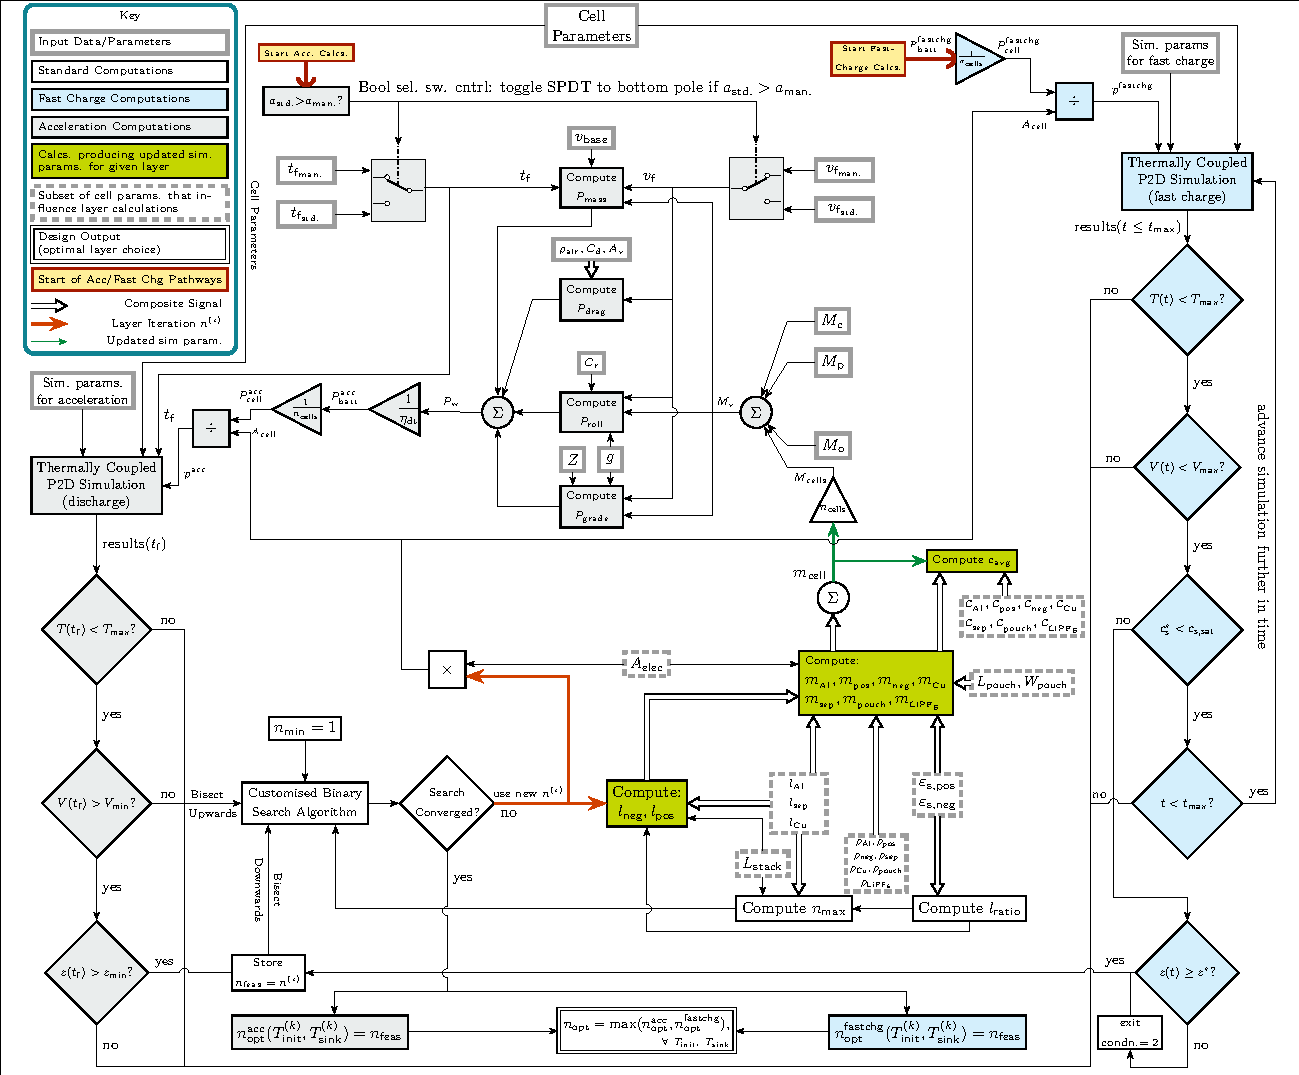
\includegraphics[angle=90, width=\textwidth]{fig_master_flow_diagram}
        \caption
        [%
        Flow diagram depicting an overview of the proposed layer optimisation methodology
        for Li-ion pouch cells.
        ]%
        {%
            Flow diagram depicting an overview of the proposed layer optimisation methodology
            for Li-ion pouch cells\footnotemark.
        }%
        \label{fig:fig_strategy_schematic}
        \mpfootnotes[1]
        % \vspace*{1.125cm}
        \vspace*{0.7225cm}
        \footnote{This figure was created by \mbox{Krishnakumar Gopalakrishnan} who
            asserts copyright, with intellectual contributions from and the right to
        use asserted by \mbox{Ian Campbell}.}
    \end{minipage}
\end{figure}
\section{Results}\label{sec:resultslayeropt}
\section{Common Module Design}\label{sec:commonmodulelayeropt}
\section{Modification of Standard \glsfmtshort{dfn} Model to Handle Power Inputs}\label{sec:innatepowerinput}

%Impart knowledge on energy cell versus power cell with the help of a diagram.
%Explain the effect of useable energy and power for a given cell with the help of
%a figure and table. How layers place a role in controlling this trade-off shall
%be discussed in the subsequent sections.

%\section{Augmentation of p2d parameters}

%Shed more light on the p2d model. Explain how they do not model a cell of given
%capacity, but instead work on a  normalised basis driven by the applied current
%densities rather than the external current.  The parameter that layers within a
%cell  change  is the  overall  electrochemically  active cross-sectional  area.
%Criticise  how published  literature  curiously omit  this important  geometric
%parameter, however  they may be  forgiven in the scope  of their work  since it
%needs only normalised dynamics. This  parameter comes into light when modelling
%anything  involving geometries  as  in this  project. This  is  the product  of
%surface area per face  and the number of layers. To  determine the surface area
%per face, the author has derived a new methodology/process involving a sequence
%of  steps, based  on assumptions  and literature  search. The  process involves
%selection of a  real-world cell, and ultimately mapping it  to the surface area
%per  unit face.  To the  best  knowledge of  the  author, this  mapping from  a
%physical cell to the Newman model is  unique and is claimed as the author's own
%contribution to the art.

%Describe briefly  the process of  mapping a  real-world cell onto  the standard
%\gls{p2d} model.

%Note: Krishna wrote the Northrop to EV mapping code and explained the concept to
%the mapping to Ian. Ian's help on the matter is identified where relevant.

%\subsection{Modelling Platform and Preconditioning}

%Couple of statements about why LIONSIMBA was chosen as the modelling platform
%for implementing the p2d dynamics. The cell parameters used are shown in table
%xx. This cell is henceforth known as the LIONSIMBA cell or Northrop cell.

%Discuss the missing elements in LIONSIMBA only with respect to the present
%problem at hand, \viz{the stoichiometries}. Thanks to Ian for running the
%time-intensive and memory-intensive simulation process on his workstation and
%offering comments on datalogging.

%\subsubsection*{Stoichiometry Augmentation}
%Discuss the problem first. How LIONSIMBA started always at 85.51 percentage and
%needed to do a discharge down to zero percent before having the ability to
%charge. For this project, stoichiometries are vital for capacity determination
%and the 1C current density. Explain how stoichiometries were refined until
%cut-off for infinitesimal bleeding discharge current achieved. Noted relevant
%values. Explanation with detailed figure on how stoichiometries were found to be
%missing. Explain refinement of how approximate capacities reported by Northrop
%and Subramanian were refined precisely. Explanation of remnant capacities and
%stoichiometries computation. Explanation of 1C current density. Note: Krishna
%wrote the parameters init capacity computation code. Thanks to Ian for running
%the simulation

%\subsection{Selection of a Suitable Reference Capacity Cell}

%Explanation of how the Bolt EV cell was selected (state of the art in driving
%range) In particular, explain how the critical computation of 60 Ah capacity was
%done. Furthermore, convincingly explain how a pouch cell thickness of 10 mm was
%used with all the background references.

%Note: Krishna did this thorough literature review, whose proof is available with
%timestamp in Box. Krishna would like to thank Ian for his time in brainstorming
%the exact BEV to use. This phase lasted a couple of weeks. For the PHEV, Krishna
%and Ian jointly did the PHEV literature search, and since Krishna does not
%intend to go in depth for PHEV results, Ian may choose to use it and simply
%acknowledge Krishna.

%\subsection{Layer Assembly within Pouch Cells}
%With the help of Northrop's layer assembly figure, explain the layer
%configuration/arrangement within a pouch cell. The next task is then identified
%as computing the number of layers within the pouch cell.

%\subsubsection*{Number of Layers of LIONSIMBA aka Northrop cell}
%Krishna came up with the idea of using integer optimisation for this task. The
%software MIDACO was also selected by Krishna and explained to Ian. The MIDACO
%result of the number of layers within the standard cell was now available.

%\subsubsection*{Computation of Surface Area per face, \protect{$A_\text{cell}$}}
%Show the simple algebraic computation of overall surface area $A$ and the
%per-face area $A_\text{cell}$. Explain how the area per face shall be a key
%quantity in the layer optimisation framework discussed later on.

%Layerphoto showing face areas and anode/cathode verhand etc will be shown here

%This concludes the augmented set of parameters added by the author to the basic
%parameter set of the DFN model. The added numerical value of parameters are
%summaried in table xx. Lots The layer optimisation framework and assumptions is
%described next. % table: pouch length, width, tab area, stack thickness etc.

%\section{Layer Optimisation Framework}

%Basically the pack configuration and the universe in which we worked shall be
%discussed here with the help of the hierarchical powertrain-to-cell schematic.
%This will set the context of the problem being tackled. Important concepts that
%enable the creation of the universe in which we define the problem to be solved
%in discussed and the assumptions involved shall be explained.

%The layer optimisation framework hinges upon the concept of capacity balancing
%between electrodes. Explain this nicely with references and citations on why
%this is important. Helps us make us of the most of the active material invested
%into the cell.


%\subsection{Capacity Balancing}
%Formula for capacity balance. Show how the length of the negative electrode is
%slightly larger than the positive electrode, but compensated for by the reduced
%volume fraction. Cite other parameter sets where this is observed. They are
%nearly equal, but made to be 1.10

%Note: This 1.1 ratio was fixed by Krishna. I can explain in person how
%this happened (reason: numerical convergence). The thickness of the positive
%electrode was adjusted accordingly. If Ian is asked this question and details of
%its origin, Krishna is sure he cannot explain it.

%\subsection{Electrode Thicknesses per layer}
%Talk briefly about separator and how its thickness remains constant.

%With this, show the mathematical derivation of the expression for number of
%layers Explain the significance of the outermost layer and how it affects the
%formula used Explain how the stack is formed. Report its numerical value. Pouch
%thickness and its role along with suitable reference. Show briefly a clever
%computer code snippet that encapsulates both cases of odd and even.

%At this stage, can explain clearly the relationship between the theoretical
%capacity and number of layers. Use a graph or a table to highlight the
%idea. Useable capacity shall be lower than total capacity due to cutoff
%considerations. Explanation.

%Note: Again, Krishna explained the layer calculation formulae to Ian.
%Especially, the derivation of the combined electrode thickness concept, and the
%usage of the ratio to obtain one from the other. Ian had to write it down
%multiple times drawing the layers and verify that my computation was correct.
%Krishna explained how the cases environment can be used for theoretical
%description while the computer code for both the cases uses ceil and floor. Ian
%naively used the mathematical symbol for ceil, until Krishna explained to him
%about the cases environment. Krishna also typed up these equations (basically
%any equation that required a derivation) in the paper manuscript.

%\subsection{Derivation of analytical \protect{$n_\text{max}$}}

%The search space spans a finite number of layers. An initial alternative
%considered was MIDACO. The detailed equations and how they are derived go here.
%Discuss for both odd and even cases. However, closed form analytical expressions
%are now available. This is so as to enable a binary search as discussed in the
%next section.

%The optimisation formula and analytical solution shall also be discussed here.

%Note: Krishna is claiming the idea generation and coding in entirety. The mixed
%integer optimisation to zero thickness was some fancy coding. The zero thickness
%idea was also quite fancy. Krishna came up with the whole of this section.
%Initiated the idea of narrowing down the search window. Ian was content with
%doing a for loop since it will also work. The optimal layer in this case is the
%earliest choice of $n$ in the for loop for which the termination conditions are
%correctly satisfied. Krishna was always in favour of an optimisation approach
%from the beginning.

%\subsection{Customised Binary Search}

%A bi-section based algorithm. Algorithm/binary tree based description with
%figure/algo. Discuss the O(log n) speedup.

%Note: One fine evening, Krishna increased the computational speedup by two orders of magnitude. Proof in github and email. While Ian was always interested in a for-loop approach right from beginning, Krishna always suggested to use an optimisation approach.

%\subsection{Mass recomputation as a function of layers}
%Explanation with graph.

%\subsection{Specific-heat recomputation as a function of layers}
%Suitable explanation and plot.

%Note: Ian congratulated Krishna for mass and specifc heat computation. In his
%words, ``You were clever coming up with a scheme wherein mass varies as a
%number of layers''. Packaged this up as a function and all. Refer to
%computelumpedmassandCpavgforgivenlayerfcn. Can prove git history for this file.
%Not only mass recomputations but also mass initial computation was done by
%Krishna

%\subsection{Thermal space permutation of layers.}
%Explanation of how the four corner temperatures are tried here. 5 lines of code snippet that packs a punch

%Note: Krishna read the acceleration specification description,educated Ian and implemented this.

%\begin{quotation}
%Ian: Krishna!. Whoa that small block of code does so much.
%\end{quotation}

%\section{Workflow for Optimal Layer Computation}

%This section discusses the actual methodology or the procedure in which the
%aforementioned ideas are incorporated in a process-like workflow. Introduce the
%full-page crazy flow diagram here. Explain how the flow diagram goes through a
%methodical approach in arriving at the optimal number of layers. Extensive
%forward and backward referencing to sections discussing each modular idea
%encountered in the flow path. Discuss how the applied current and power
%densities change due to change in overall surface area while the applied
%external current/power remains the same.

%% This will help us to apply current in units rather in current density.

%The salient cases to be covered are the following.

%\subsection{Case 1 --- Analysis of Drivecycle Powers}

%Although from Colorado Boulder lecture notes, Krishna already knew that
%acceleration demands the highest power demand on the cell, it needs to be proven
%that drive cycles, which are the basis for various fuel efficiency calculations
%do not represent this case. Ian did the comparative study of various drivecyles.
%Some plots and charts showing various power levels were generated by him.
%Krishna does not explicity need to use this section, and is optional to the
%story, other than the sake of well-roundedness and demonstrating thoroughness of
%the study.

%Explain that this case is not present in the flow diagram.

%However, it was Krishna who generated the drivecycle speed vs time and
%acceleration versus time results alone and then informed Ian afterwards that it
%is now available in the repository. If Ian uses this section, an acknowledgement
%will be appropriate.


%\subsection{Case 2 --- Acceleration from standstill}

%Explanation and computations based on standard vehicle dynamics. Lecture notes
%and videos given to Ian by Krishna from Univ of Colorado Boulder The sole value
%addition in this case is the specification to adhere to and its implementation
%through a cases study. Krishna shall explain this through either-or if-then
%case, explanation along with a short code snippet which he implemented alone.

%Explain the acceleration run in detail, what it entails etc. Walk through the
%flow diagram till acc layer results are discussed.

%Note: The acceleration specification for electrified transport was unearthed by
%Krishna (all the interlibrary loan stuff and educated Ian about it). Two
%passengers and all that thing. Complete coding.

%\subsection{Case 3 --- Fast Charging}

%A brief explanation of the whys and the hows and implications. Explanation of
%prevalent standards. Present table of standards etc etc

%One paragraph review of control algorithms and how this algorithm was chosen.
%Brief overview of algorithm. The idea of introducing saturation and pulsed
%charging profile. Based on patent at Auburn university. Krishna did literature
%review. Flag introduced in code. Code snippet.enablecsnegsaturationlimit.
%% Sinusoidal excitation charging.

%Explanation of why power demand is important (based on charger power electronics).
%Finally, walk through of the fast charging section of the schematic.

%Note: Krishna performed the litt search of this section entirely (proof with
%timestamp available). However, Krishna is tentatively not using a detailed litt
%review. In kind consideration of Ian's own overarching thesis topic, which
%Krishna understands to be something pertinent to fast charging, Krishna can let
%Ian use the literature provided proper attribution is in place. For the sake of
%completion, the MIDACO based approaching to fast charging showing the pulsing
%power is also possible by Ian (just a suggestion).

%Note: The charger power electronics limit is again my contribution from an EEE
%background

%% \item Review of model-based fast charging control algorithms (how does this go into litt review)

%\section{Simulation Environment}
%Discuss parameters of simulation environment. Discuss with the help of a table
%for the BEV case only. Ian can take the PHEV Number of BEV calls designed to
%make up the series string.

%Krishna also came up with the cell's cutoff study with respect to the the
%system's bus bar voltage, and will be cited here with examples and strong
%backing. There are a few preconditioning steps needed to amend the p2d model
%before numerical implementation of the flow diagram is possible. 1. Fixing
%aspects of the code in LIONSIMBA v1.023 used as the baseline by this thesis
%author. 2. Addition of the capability to apply power input instead of current
%input as is common in traditional p2d simulations.

%Note: All crucial parameters were sourced by Krishna through a literature
%review. Especially, the vehicular parameters like classis mass, coefficient of
%drag, base speed. Krishna also had to educate Ian about base speed. If an on the
%spot quiz is conducted at a conceptual level, this truth can easily be deduced
%by the judging authority. Krishna claims the literature review of this topic and
%is happy to let Ian use this with proper attribution.

%\subsection{Preconditioning of Computer Code}

%Briefly allude to the stoichiometries that was introduced into the computer code
%through capacity characterisation simulation.Now possible to start at any SoC.
%The other salient amendments and enhancements to the software toolbox is shown
%below. Released as 2.0 and link to LIONSIMBA github repo (not BOLD toolbox repo)

%\subsubsection{Re-parameterisation}

%Discuss the extensive Reparameterisation undertaken by Krishna by studying
%relevant literature. Discuss the changed parameters with respect to Northrop
%cell and why. Maybe show a table. This is quite substantial.

%Conductivity/diffusivity changes. Show how the isothermal and thermal variants
%in existing Northrop cell were bogus with plots.

%Performed comprehensive literature review to replace the dubious/bogus
%parameters of the electrode and electrolyte specific heat capacities email proof
%PS: Every thermal/material property of the Al/Cu current collectors is very
%clear and have been traced out, hand-calculated and validated.

%\subsubsection{Deterministic initialisation of algebraic variables}

%Replaced silly fsolve. Numerical explanation here.

%\subsubsection{Linear interpolation for field variables}

%Explain how linear interpolation was performed for phis and phie at the edges
%of control volumes in electrode and separator. Draw a schematic for this
%explanation.

%\subsubsection*{Convergence Analysis of Computation Mesh}
%Report only if Krishna has sufficient time left. Explain simplifying
%assumptions. Refer to the table etc Show plot of how terminal voltage is
%converging for chosen mesh as a function of number of nodes. Another plot of how
%simulation end time converges as a function of number of nodes. Lots of analysis
%by changing the number of nodes within each mesh to justify the validity of the
%results. Prove that mesh independence is reached.

%\subsection{Hybrid fv--Spectral Scheme}

%Completely numerical section. Highly mathemetical. Explain how the rational to
%decimal truncation of the unbalanced twelfth order finite difference scheme
%messes up numerical conditioning. Show matrices and discuss the drawbacks.
%Fornberg matrix did not help. So, spectral scheme was needed.

%Background study, explanation, analysis, literature review and equation
%derivation of spectral scheme Complete contribution of solid-phase diffusion
%with spectral methods. Reading textbook, understanding concept, investigation of
%applicability, hunting relevant literature, text-writing, hand-derivation of
%equations. This complete section was done by Krishna.

%\subsection{Lumped Thermal Model}

%Basic discussion of lumped thermal model and justify through citations why here
%it might be sufficient for this application. Not originally present in
%LIONSIMBA. Present the thermal model here equations here. Discuss what cp avg
%means and how it is computed as a here function of number of layers. Explanation
%of how tab cooling helps here.

%Note: Cp avg was calculated and coded by Krishna, as a function of number of
%layers. I shall leave the detailed thermal model to Ian, especially since a biot
%analysis was performed by him. Anyway, suddenly discussing the thermal model at
%depth does not fit the story of my thesis. My hint to Ian would be to emphasise
%the thermal model at depth, since anyway he seems to be confident in the biot
%analysis. Specifically the value of heat transfer coefficient was empirically
%chosen by Ian through simulations. So, I will let him explain that stuff.
%However, tab area idea computation using twice the Bolt's tab area was proposed
%by Krishna, but overall this thermal stuff, Krishna is willing to bequeath to
%Ian since the whole thing doesn't fit the story of Krishna's work. The
%polarisation heat concept was initially described by Greg, but anyway let Ian
%explain it, no problem. Ian may wish to discuss entropic heat generation and a
%lot of other things we investigated together, but I am not going to dwell on
%them in the thesis.


%\subsection{Power Input Boundary Conditions}

%Discuss why power input is needed for layer optimisation. Explain how it is done
%currently in state of the art case.

%Krishna educated Ian about Pletts existing work. Accompanied Ian to the library
%and told him to check out that book which I had ordered.

%Krishna claims a very important thing here. A critical argument on how the
%present schemes do not fit into the layer opt methodology.

%Detailed mathematical derivation. Both Ian and Krishna acknowledge each other's
%help in shared derivation and also acknowledge Davide appropriately.

%Note: Ian might wish to report the two intermediate steps before this solution
%was obtained. The 2nd of the 3 approaches was matching current and voltage at
%discrete intervals through numerical integration. This was our third approach.
%The first approach was too simplistic. So, Ian might wish to skip it.



%\section{Layer Optimisation Results}

%Show the table only with the extra parameters not present in isothermal model.
%In particular, I can remember the thermal parameters of the two electrodes,
%separator, pouch, current collectors and electrolyte.

%Present the results in a horribly bland table format steering well clear of the
%heatmap. Krishna's view is that the results do not stand alone by themselves and
%if you plonk a layer choice from the heatmap/table into your cell, things are
%not expected to work as is. The numbers herein are the result of quite a few
%assumptions and hold validity only within the universe in which it was created.

%However, the framework itself is transferable and is the most valuable component
%of the work. A user reading this thesis can easily substitute their own cell
%parameters and system-level considerations into the code and obtain results from
%it accordingly. This was the working premise of the paper as well, until Ian
%decided to write up a bloated explanatory section.

%Plots of acceleration and fast charging for successful layer count.

%For PHEV, although common module design will be alluded to, it will not be dwelled on or explained or analysed in depth.


%Note: In Ian's thesis, Krishna seeks attribution for the idea to use a heatmap
%since it arose out of Krishna's heavy criticism, bordering on the offensive,
%about continuously complaining that our group's plots/charts/graphs do not
%exhibit any ``interesting'' twists and turns and fancy illustrations. Apologies
%for this. Anyway, the heatmap idea was my suggestion. However, I shall not take
%an inch of credit for the implementation as it was entirely Ian's work in coming
%up with fancy schemes.

%Note: Having obtained BEV results, Krishna also set up the full set of
%assumptions for the PHEV simulations too before leaving actual numerical
%simulations to Ian (and on vacation to India followed by Konstanz). So an
%acknowledgement is required if Ian choses to list these assumptions. Ian can
%discuss monotonicity issues in PHEV simulation that he found out about.

%\section{Appendix}

\section{Lower Cutoff Voltage}\label{sec:cutoff}
% -*- root: ../../main.tex -*-
%!TEX root = ../../main.tex
% vim:nospell

\begin{table}[!htbp]
    \small
    \caption[%
    System-level simulation conditions \& thermal parameters of  an \glsfmtshort{lco} cell
    ]%
    {%
        Cell   parameters   and   system   conditions  for   a   simulating   an
        \glsfmtshort{lco} cell  with the  \gls{dfn} electrochemical model  and a
        lumped thermal model. The parameters  presented here when augmented with
        the  values  of  the  kinetic, geometric  and  transport  properties  of
        the  cell (from  \cref{tbl:lcoSimParamsSPMp2d}  represents the  complete
        information  required for  all  simulations in  this layer  optimisation
        framework.
    }%
    \label{tbl:lcoSimParamslayeropt}
    \vspace{-2.6229525pt}
    \begin{threeparttable}
        \centering
        \textbf{System Conditions} \\ \smallskip
        \begin{varwidth}[t]{0.48\linewidth}
            \begin{tabular*}{\textwidth}{@{} l @{\extracolsep{\fill}} S[table-format=1.2,table-space-text-pre=\Tnote{a} ,table-align-text-pre=false] @{}}
                \toprule
                \multicolumn{1}{@{}l}{Parameter} \\
                \midrule

                Lower cutoff cell voltage, $V_\text{min}$ (\si{\volt}) & \Tnote{a} 3.50   \\
                Upper cutoff cell voltage, $V_\text{max}$ (\si{\volt}) & \Tnote{b} 4.22   \\

                \bottomrule
            \end{tabular*}
        \end{varwidth}
        \hfill
        \begin{varwidth}[t]{0.48\linewidth}
            \begin{tabular*}{\textwidth}{@{} l @{\extracolsep{\fill}} S[table-format=2.2,table-space-text-pre=\Tnote{a} ,table-align-text-pre=false] @{}}
                \toprule
                \multicolumn{1}{@{}l}{Parameter} \\
                \midrule

                Target cell SOC for fast charge, $z^\ast$ \si{(\%)}                & \Tnote{c} 80.00 \\
                Cell upper temperature limit, $T_\text{max}$ \si{(\degreeCelsius)} & \Tnote{d} 55.00 \\

                \bottomrule
            \end{tabular*}
        \end{varwidth}

        \medskip
        \begin{tabular*}{\textwidth}{@{} l @{\extracolsep{\fill}} r @{}}
            \multicolumn{2}{c}{\textbf{Geometric Parameters}} \\
            \toprule
            \multicolumn{1}{@{}l}{Parameter} \\
            \midrule
            Surface area of pos.\ \& neg.\ electrode overlap within a layer, {$A_\text{elec}$} \si{(m^2)} & \textsuperscript{b}\num{4.19e-2}   \\
            Exterior pouch length, $L_\text{pouch}$ \si{(m)}                                              & \textsuperscript{e}\num{332.74e-3} \\
            Exterior pouch width, $W_\text{pouch}$ \si{(m)}                                               & \textsuperscript{e}\num{99.06e-3}  \\
            Exterior pouch height, $H_\text{pouch}$ \si{(m)}                                              & \textsuperscript{f}\num{10.00e-3}  \\
            Pouch material thickness, $T_\text{pouch}$ \si{(m)}                                           & \textsuperscript{g}\num{160.00e-6} \\
            \bottomrule
        \end{tabular*}
        \medskip
        \centering \textbf{Thermal Parameters} \\ \smallskip
        \resizebox{\textwidth}{!}{%
            \begin{tabular}{@{} l S[table-format=4.0,table-space-text-pre=\Tnote{m} ,table-align-text-pre=false] S[table-format=4.1,table-space-text-pre=\Tnote{m} ,table-align-text-pre=false] S[table-format=4.1,table-space-text-pre=\Tnote{m} ,table-align-text-pre=false] S[table-format=4.2,table-space-text-pre=\Tnote{m} ,table-align-text-pre=false] S[table-format=4.0,table-space-text-pre=\Tnote{m} ,table-align-text-pre=false] S[table-format=4.1,table-space-text-pre=\Tnote{m} ,table-align-text-pre=false] S[table-format=4.1,table-space-text-pre=\Tnote{m} ,table-align-text-pre=false] @{}}
                \toprule
                \multicolumn{1}{@{}l}{Parameter} & \multicolumn{1}{c}{Al.\ CC} & \multicolumn{1}{c}{Pos} & \multicolumn{1}{c}{Sep} & \multicolumn{1}{c}{Neg} & \multicolumn{1}{c}{Cu.\ CC} & \multicolumn{1}{c}{\ch{LiPF_6}} & \multicolumn{1}{r@{}}{Pouch}\\
                \midrule

                Sp.\ heat capacity, $c_j$ (\si{\joule\per\kilogram\per\kelvin})   & \Tnote{h} 903  & \Tnote{h} 1269.2 & \Tnote{h} 1978.2 & \Tnote{h} 1437.4 & \Tnote{h} 385  & \Tnote{h} 2055.1 & \Tnote{i} 1464.8 \\
                Density, $\rho_j$ (\si{\kilogram\per\meter\cubed})                & \Tnote{j} 2700 & \Tnote{k} 2291.6 & \Tnote{b} 1100.0 & \Tnote{j} 2660.0 & \Tnote{l} 8960 & \Tnote{j} 1290.0 & \Tnote{m} 1150.0 \\
                Activ.\ energy, diff. ${E_\text{act,s}}_j$ (\si{\joule\per\mole}) & {---}                   & \Tnote{p} 5000   & {---}                     & \Tnote{p} 5000   & {---}                   & {---}                     & \multicolumn{1}{c}{---}   \\
                Activ.\ energy, rxn. ${E_\text{act,k}}_j$ (\si{\joule\per\mole})  & {---}                   & \Tnote{p} 5000   & {---}                     & \Tnote{p} 5000   & {---}                   & {---}                     & \multicolumn{1}{c}{---}   \\

                \bottomrule
            \end{tabular}
        }
        \medskip
        \begin{tabular*}{\textwidth}{@{} l @{\extracolsep{\fill}} r @{}}
            \multicolumn{2}{c}{\textbf{Other Geometric/Cell-Level Parameters}} \\
            \toprule
            \multicolumn{1}{@{}l}{Parameter} \\
            \midrule

            Thickness of pos.\ current collector, $l_\text{Al}$ \si{(m)}                    & \textsuperscript{f}\num{15e-6}   \\
            Thickness of neg.\ current collector, $l_\text{Cu}$ \si{(m)}                    & \textsuperscript{p}\num{10e-6}   \\
            Total tab area, $A_\text{tabs}$ \si{(m^2)}                                      & \textsuperscript{b}\num{5.94e-3} \\
            Lumped heat transfer coefficient, $h$ (\si{\watt\per\meter\squared\per\kelvin}) & \textsuperscript{b}150           \\
            Initial electrolyte concentration, $c_\text{e,0}$ (\si{\mole\per\meter\cubed})  & \textsuperscript{q}1000          \\

            \bottomrule
        \end{tabular*}

        \medskip
        \begin{tabular*}{\textwidth}{@{} =P{7.5cm}  +l@{\extracolsep{\fill}}+c +r @{}}
            \multicolumn{4}{c}{\textbf{Spatial Discretisation}} \\
            \toprule
            \multicolumn{1}{@{}l}{Parameter} & \multicolumn{1}{l}{Pos} & \multicolumn{1}{c}{Sep} & \multicolumn{1}{r@{}}{Neg}\\
            \midrule

            Nodes, through-thickness (axial), $N_{\text{a}_j}$          & \num{40} & \num{40} & \num{40} \\
            Nodes, within spherical particle (radial), $N_{\text{r}_j}$ & \num{15} & ---      & \num{15} \\

            \bottomrule
        \end{tabular*}

        \medskip
        \vspace{-2.6229525pt}
        \begin{tablenotes}[para,flushleft]
            \begin{footnotesize}
            \item[a] Calculated as described in \cref{sec:cutoff}
            \item[b] Assumed
            \item[c] Ref.~\cite{Sae2010}
            \item[d] Ref.~\cite{Kizilel2009} \\
            \item[e] Converted from imperial units reported in~Ref.~\cite{GMBoltBatteryDims}
		    \item[f] Table~\romanletter{4} of~Ref.~\cite{Groger2015} \\
            \item[g] Sum of values in table~1 of~Ref.~\cite{Svens2013}
            \item[h] Ref.~\cite{Chen2005}
            \item[i] Computed from values of constituents (see~\cite{Svens2013}) using Ref.~\cite{martienssen2006springer} \\
            \item[j] Ref.~\cite{Guo2010}
            \item[k] Ref.~\cite{Jeon2011}
            \item[l] Ref.~\cite{Worwood2017,Song2000}
            \item[m] Ref.~\cite{Kim2009}
            \item[p] Ref.~\cite{Northrop2011}
            \item[q] Ref.~\cite{Subramanian2009}
            \end{footnotesize}
        \end{tablenotes}
    \end{threeparttable}
\end{table}



Figure showing power input

\section{Hybrid Spectral-\glsfmtshort{fv} Scheme}\label{sec:hybridfv-spectral}

Fast  and  accurate  estimation  of   the  solid  phase  lithium  concentration,
particularly  its   value  at   the  surface  of   electrode  particles   is  an
inherent  requirement   of  the   layer  optimisation  procedure   presented  in
Section~\ref{sec:layeroptframework}.  The  high   power  densities  that  result
from  using  low  layer  counts   necessitate  this  requirement.  It  has  been
acknowledged that concentration calculations employing polynomial approximations
such  as   those  proposed   in~\cite{Santhanagopalan2006a}  lack   fidelity  at
high  charge/discharge rates~\cite{Santhanagopalan2006}.  Hence, a  conventional
full-order solution based on Fick's law of diffusion is appropriate.

With full-order solid phase diffusion dynamics, applying the \gls{fv} scheme
(that has been employed to discretise all through-thickness \gls{pde}s in the
\gls{p2d} model) results in a large system of equations. This is due to the
requirement of using a high radial node density per spherical particle
for improved accuracy. Consequently, the computational cost is high and
simulation runtime becomes prohibitive when exploring the search space of
all possible layer configurations. Moreover, with a cell-centered \gls{fv}
discretisation, it is non-trivial to directly apply the ionic flux boundary
condition at the particle surface, since it involves extrapolation from at
least two other nodes within the particle. While such extrapolations are
acceptable in the axial dimension --- particularly with high node densities
providing small values of $\frac{\Delta x}{2}$ --- they are undesirable in
the radial dimension. This is because cell's open circuit and terminal
voltages strongly depend on the concentration at the particle surface. Spectral
methods offer a combination of high accuracy and speed while permitting
the use of a lower number of radial discretisation nodes. To implement a
spectral scheme on a non-periodic domain, a Chebyshev discretisation may be
applied~\cite{Trefethen2000}. Bizeray~\etal discretised all of the \gls{p2d}
model equations using this approach~\cite{Bizeray2015a}. However, this entails a
bi-directional mapping of all variables between the physical and Chebyshev
domains, incurring computational overhead.

Here we propose the use of a hybrid formulation of the \gls{p2d} model wherein a
standard \gls{fv} scheme in the axial dimension and a spectral scheme in the
radial domain are used. By exploiting the natural separation of the axial and
radial domains, we \romanletter{1}) retain the ability to easily couple the
molar flux density at the particle surface through reformulation of the
boundary conditions of the solid diffusion pde and \romanletter{2}) solve for
solid-phase lithium concentration in the Chebyshev domain and locally transform
to physical domain, without requiring system-wide Chebyshev reformulations.
Although the proposed implementation does not globally employ a spectral
scheme, the combined beneficial effects of radial-domain spectral scheme and
automatic differentiation of system equations using CasADi~\cite{Andersson2013b}
facilitates rapid simulation, enabling layer optimisation on short time-scales.
Eqns\cref{eqn:defineChebNodes}--\cref{eqn:solidDiffEqChebDomain} detail the
steps leading to the reformulated solid phase diffusion and its associated
boundary condition in the Chebyshev domain.

The Chebyshev collocation nodes defined on a 1D mesh in the radial direction are
given by\cref{eqn:defineChebNodes}~\cite{Trefethen2000}.

\begin{equation}\label{eqn:defineChebNodes}
    \tilde{r} = \cos\left(\frac{i\pi}{N_\text{r}}\right), \qquad i = 0, 1, \dots N_\text{r} \quad \tilde{r} \in [-1, 1]
\end{equation}

Assuming constant diffusivity, and expanding the derivative in the standard
form of the Fickian spherical diffusion equation for each particle
(refer~\ref{sec:Supplementary}) we obtain \cref{eqn:quotientappliedpde},
presented along with its Neumann boundary conditions. $j$ is the molar flux
density (\si{mol.m^{-2}.s^{-1}}) and $R_\text{p}$ is the particle radius
(\si{m}).

\begin{align}
    \frac{\partial c_\text{s}}{\partial t} &= D^\text{eff}_\text{s} \left( \frac{\partial}{\partial r} \frac{\partial c_\text{s}}{\partial r} + \frac{\partial^2 c_\text{s}}{\partial r^2} \right) \qquad r \in [0, R_\text{p}]\label{eqn:quotientappliedpde}\\
\frac{\partial c_\text{s}}{\partial r}\bigg\rvert_{r=0} &= 0\tag{\ref{eqn:quotientappliedpde}a}\\
 D^\text{eff}_\text{s}\frac{\partial c_\text{s}}{\partial r}\bigg\rvert_{r=R_\text{p}} &= {}-j\tag{\ref{eqn:quotientappliedpde}b}
\end{align}

{Mapping} $r \in [0,R_\text{p}] \mapsto \tilde{r} \in [-1, 1]$,
\begin{align}\label{mappingChebDomain}
    r = \frac{R_\text{p}}{2}(\tilde{r} + 1)
\end{align}

Applying \cref{mappingChebDomain} to \cref{eqn:quotientappliedpde}
whilst retaining $c_\text{s}$ in the physical space yields
\cref{eqn:solidDiffEqChebDomain}.

\begin{align}
	\frac{\partial c_\text{s}}{\partial t} &= 4 \frac{D^\text{eff}_\text{s}}{R_\text{p}^2} \left( \frac{2}{\tilde{r} + 1} \frac{\partial c_\text{s}}{\partial \tilde{r}} + \frac{\partial^2 c_\text{s}}{\partial {\tilde{r}}^2} \right)\label{eqn:solidDiffEqChebDomain}\\
\frac{\partial c_\text{s}}{\partial \tilde{r}}\bigg\rvert_{\tilde{r}=-1} &= 0\tag{\ref{eqn:solidDiffEqChebDomain}a}\\
	2 \frac{D^\text{eff}_\text{s}}{R_\text{p}} \frac{\partial c_\text{s}}{\partial \tilde{r}}\bigg\rvert_{\tilde{r}=1} &= -j\tag{\ref{eqn:solidDiffEqChebDomain}b}
\end{align}

During the iterative solution process, the spatial gradients of solid phase
lithium concentration in \cref{eqn:solidDiffEqChebDomain} are not computed
through an explicit differentiation procedure, but instead evaluated by
pre-multiplying the concentration values at the collocation nodes by a
Chebyshev differentiation matrix. This particular fact is responsible for
the inherent reduction of simulation runtime achieved by introducing a
spectral method. In the modified version of LIONSIMBA used in the layer
optimisation methodology, differentiation matrices of suitable dimension as well
as the Chebyshev collocation nodes are generated using the MATLAB function
\texttt{cheb.m}~\cite{Trefethen2000}.

% Intend to provide a call-graph in the appendix



% -*- root: ../../main.tex -*-
%!TEX root = ../../main.tex
% vim:nospell


\begin{table}[!htbp]
	\renewcommand{\thetable}{\arabic{table}a}
	\centering
	\caption{Acceleration test parameters (common across xEV platforms)}
	\label{tbl:CommonVehicleParams}
	\sisetup{table-format=3.2, table-number-alignment=center, table-space-text-pre=\textsuperscript{a}, table-space-text-post=\textsuperscript{a}, table-align-text-post=false}
	\begin{threeparttable}[t]
		\centering
		\begin{tabular}{@{} l  S @{}}
			\toprule
			Parameter \\
			\midrule

			% Coefficient of drag for xEV body, $C_\mathrm{d}$                           & {\makebox*{00}[r]{\tnote{a}}} 0.31                \\
			% Frontal area of xEV, $A_\mathrm{v}$ \si{(m^2)}                             & {\makebox*{00}[r]{\tnote{b}}} 2.40                \\
			% Acc.\ time specified by manufacturer, $t_\mathrm{f,man}$ \si{(s)}          & {\makebox*{00}[r]{\tnote{d}}} 6.50                \\
			% Acc.\ time dictated by standards, $t_\mathrm{f,std}$ \si{(s)}              & {\makebox*{00}[r]{\tnote{c}}} 6.00                \\
			% Speed, end of acc. (standards), $v_\mathrm{f,std}$ \si{(m.s^{-1})}         & {\makebox*{00}[r]{\tnote{e}}} 8.94                \\
			% Speed, end of acc. (manufacturer), $v_\mathrm{f,man}$ \si{(m.s^{-1})}      & {\makebox*{0}[r]{\tnote{f}}} 26.82                \\
			% Base speed of  xEV, $v_\mathrm{b}$ \si{(m.s^{-1})}                         & {\makebox*{\hspace*{0.5mm}0}[r]{\tnote{e}}} 13.41 \\
			% Air density at acc.\ test conditions, $\rho_\mathrm{air}$ \si{(kg.m^{-3})} & {\makebox*{\hspace*{0.5mm}00}[r]{\tnote{f}}} 1.20 \\
			% Drivetrain efficiency, $\eta_\mathrm{dt}$                                  & {\makebox*{00}[r]{\tnote{g}}} 0.75                \\
			% Payload, $M_\mathrm{p}$ \si{(kg)}                                          & {\hspace*{0.00005mm}{\tnote{c}}} 150.60 \\
			% Rolling resistance coefficient of road surface, $C_\mathrm{r}$             & {\makebox*{00}[r]{\tnote{f}}} 0.01                \\
			% Road gradient, $Z$                                                         & {\makebox*{00}[r]{\tnote{g}}} 0.00                \\

			Coefficient of drag for xEV body, $C_\mathrm{d}$                           & 0.31   {\tnote{a}} \\
			Frontal area of xEV, $A_\mathrm{v}$ \si{(m^2)}                             & 2.40   {\tnote{b}} \\
			Acc.\ time specified by manufacturer, $t_\mathrm{f,man}$ \si{(s)}          & 6.50   {\tnote{d}} \\
			Acc.\ time dictated by standards, $t_\mathrm{f,std}$ \si{(s)}              & 6.00   {\tnote{c}} \\
			Speed, end of acc. (standards), $v_\mathrm{f,std}$ \si{(m.s^{-1})}         & 8.94   {\tnote{e}} \\
			Speed, end of acc. (manufacturer), $v_\mathrm{f,man}$ \si{(m.s^{-1})}      & 26.82  {\tnote{f}} \\
			Base speed of  xEV, $v_\mathrm{b}$ \si{(m.s^{-1})}                         & 13.41  {\tnote{e}} \\
			Air density at acc.\ test conditions, $\rho_\mathrm{air}$ \si{(kg.m^{-3})} & 1.20   {\tnote{f}} \\
			Drivetrain efficiency, $\eta_\mathrm{dt}$                                  & 0.75   {\tnote{g}} \\
			Payload, $M_\mathrm{p}$ \si{(kg)}                                          & 150.60 {\tnote{c}} \\
			Rolling resistance coefficient of road surface, $C_\mathrm{r}$             & 0.01   {\tnote{f}} \\
			Road gradient, $Z$                                                         & 0.00   {\tnote{g}} \\

			\bottomrule
		\end{tabular}
        \begin{tablenotes}[para,flushleft]
        \item[a]Ref.~\cite{HybridCars2017Drag}
        \item[b]Calculated from typical \gls{bev} dimensions in~\cite{BoltDimensions}
        \item[c]Ref.~\cite{ETANTP002-2004}
        \item[d]Ref.~\cite{BoltOverview}
        \item[e]Ref.~\cite{Liu2016a}
        \item[f]Ref.~\cite{EmadiElectric}
        \item[g]Assumed
        \end{tablenotes}
	\end{threeparttable}
\end{table}

% -*- root: ../../main.tex -*-
%!TEX root = ../../main.tex
% vim:nospell


\begin{table}[!htbp] % Parameters unique to each of the BEV & PHEV
	% \addtocounter{table}{-1}
	% \renewcommand{\thetable}{\arabic{table}b}
	\caption{Acceleration test parameters (specific to each \glsfmtshort{xeV})}
	\label{tbl:UniqueVehicleParams}
	\centering
    \sisetup{table-format=4.1, table-number-alignment=center, table-space-text-pre=\textsuperscript{a}, table-align-text-pre=false}
	\begin{threeparttable}[t]
		\begin{tabular*}{0.72\textwidth}{@{} l @{\extracolsep{\fill}}  S S @{}}	% Works with Tnote
			\toprule
			\multicolumn{1}{@{} l}{Parameter} & \multicolumn{1}{c}{BEV} & \multicolumn{1}{c@{}}{PHEV} \\
			\midrule

			Mass of xEV chassis, $M_\mathrm{c}$ \si{(kg)}               & \Tnote{a} 1340.0 & \Tnote{b} 1438.0 \\
			Mass of pack overhead (w/o cells), $M_\mathrm{o}$ \si{(kg)} & \Tnote{a} 196.4  & \Tnote{c} 65.5   \\
			Upper cutoff SOC of cell, $z_\mathrm{max}$ \si{(\%)}        & \Tnote{d} 95.0   & \Tnote{d} 90.0   \\
			Lower cutoff SOC of cell, $z_\mathrm{min}$ \si{(\%)}        & \Tnote{d} 5.0    & \Tnote{e} 30.0   \\

			\bottomrule
		\end{tabular*}
		\begin{tablenotes}[para,flushleft]
		\item[a]Calculated based on~\cite{ChevyBoltSpecs}
		\item[b]Calculated based on~\cite{motortrendEcotec,ChevyBoltSpecs}
		\item[c]Calculated (see sections~\ref{sec:layerdependentvehiclemass} \& \ref{sec:massofonecell})
		\item[d]Assumed
		\item[e]Ref.~\cite{EmadiElectric}
		\end{tablenotes}

	\end{threeparttable}
\end{table}


\section{To figure out name}\label{sec:Configurations}

% -*- root: ../../main.tex -*-
%!TEX root = ../../main.tex
% vim:nospell

\begin{table}[htb!]
    \caption{\glsfmtshort{xeV} acceleration test results}
    \label{tbl:accResults}
    \centering
	\begin{tabular}{c c c}
        \toprule
        \multicolumn{1}{@{} l}{\makecell{($T_\text{init},T_\text{sink}$) \\ \footnotesize (degC)}} & \makecell{$n^\text{acc}_\text{opt}$ \\ \footnotesize \glsfmtshort{bev}}&  \multicolumn{1}{c @{}}{\makecell{$n^\text{acc}_\text{opt}$ \\ \footnotesize \gls{phev}}}  \\
        \midrule

        (38,5)  & \num{21} & \num{55} \\
        (38,49) & \num{21} & \num{57} \\
        (25,25) & \num{23} & \num{63} \\
        (15,5)  & \num{27} & \num{69} \\

        \bottomrule
    \end{tabular}
\end{table}


\begin{figure}[!bp]
    \begin{minipage}[t]{\textwidth}
        \centering
        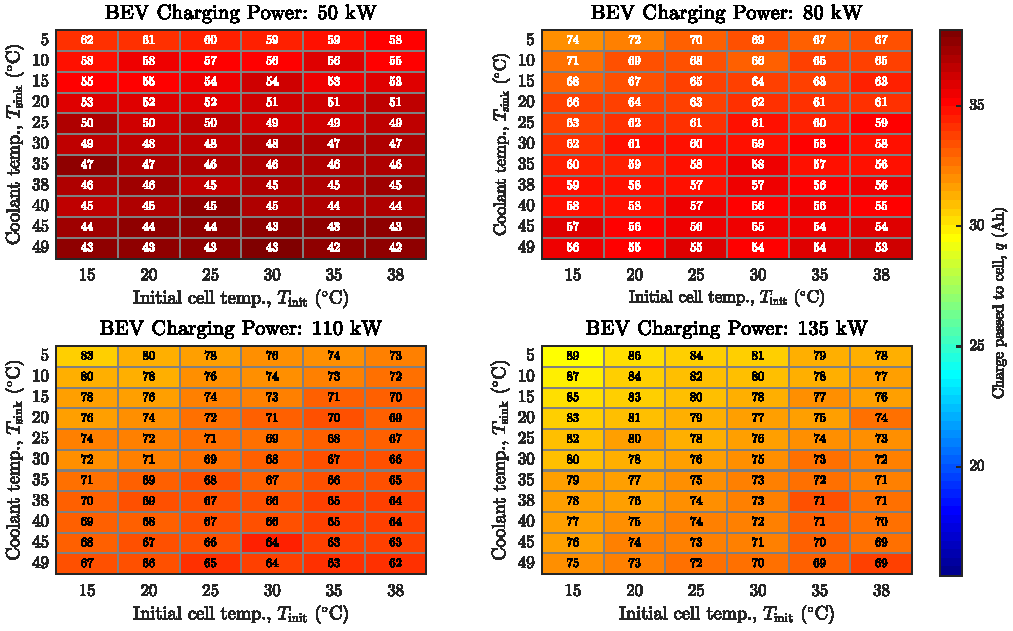
\includegraphics[width=\textwidth]{fig_generate_heatmap_BEV}
        \caption[Optimal cell layer configurations for the \gls{bev}, presented for a range of fast charging powers and thermal conditions]{Optimal cell layer configurations for the \gls{bev}, presented for a range of fast charging powers and thermal conditions\footnotemark.}
        \label{fig:fig_generate_heatmap_BEV}
        \mpfootnotes[1]
        \footnote{This figure was created by \mbox{Ian Campbell} who asserts copyright,
            with intellectual contributions from and the right to use asserted by
        \mbox{Krishnakumar Gopalakrishnan}.}
    \end{minipage}
\end{figure}

\begin{figure*}[!bp]
    \begin{minipage}[t]{\textwidth}
        \centering 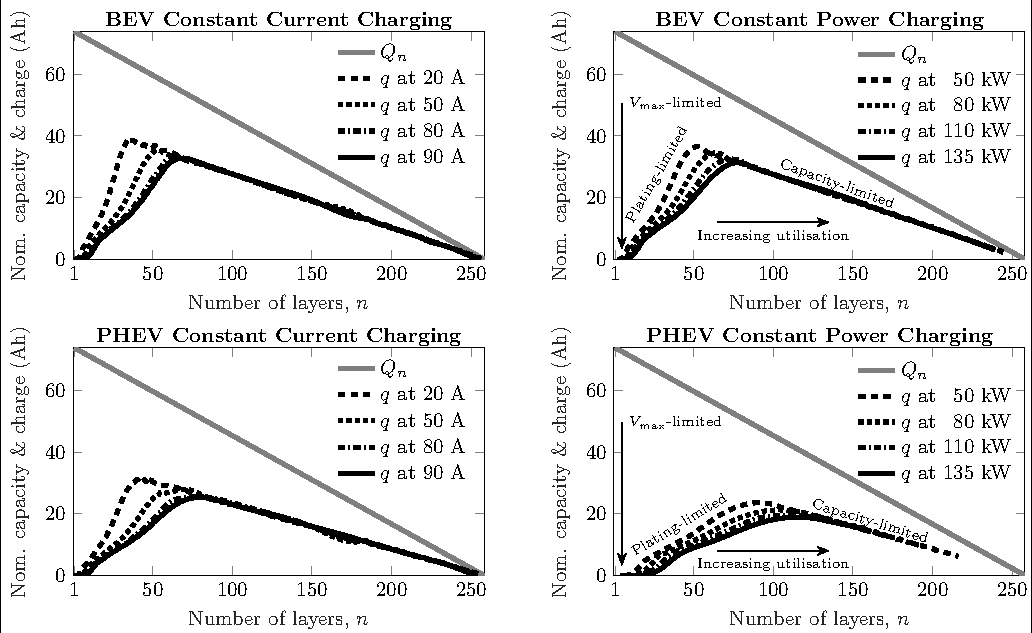
\includegraphics[width=\textwidth,trim=4 2 3 4,clip]{fig_capacity_quadrants.pdf}
        \caption[The plots in the right column show the nominal cell capacity and charge passed
        during \gls{xeV} \gls{cp} charging. Increased rate capability and cell utilisation are positively
        correlated with $n$, while the maximum-$q$ layer configuration clearly shifts to higher
        values of $n$ with increasing charging powers. The plots in the left column depict
        galvanostatic charging scenarios at various currents to highlight the similarity with the
        \gls{cp} process. All data obtained at $T_\text{init} =$ \SI{25}{\degreeCelsius},
        $T_\text{sink} =$ \SI{25}{\degreeCelsius}.]{The plots in the right column show the nominal cell capacity and charge passed
            during \gls{xeV} \gls{cp} charging. Increased rate capability and cell utilisation are positively
            correlated with $n$, while the maximum-$q$ layer configuration clearly shifts to higher
            values of $n$ with increasing charging powers. The plots in the left column depict
            galvanostatic charging scenarios at various currents to highlight the similarity with the
            \gls{cp} process. All data obtained at $T_\text{init} =$ \SI{25}{\degreeCelsius},
        $T_\text{sink} =$ \SI{25}{\degreeCelsius}\footnotemark.}\label{fig:fig_CapacityQuadrants}
        \mpfootnotes[1]
        \footnote{This figure was created by \mbox{Ian Campbell} who asserts copyright,
            with intellectual contributions from and the right to use asserted by
        \mbox{Krishnakumar Gopalakrishnan}.}
    \end{minipage}
\end{figure*}

\begin{figure}[!bp]
    \begin{minipage}[t]{\textwidth}
        \centering
        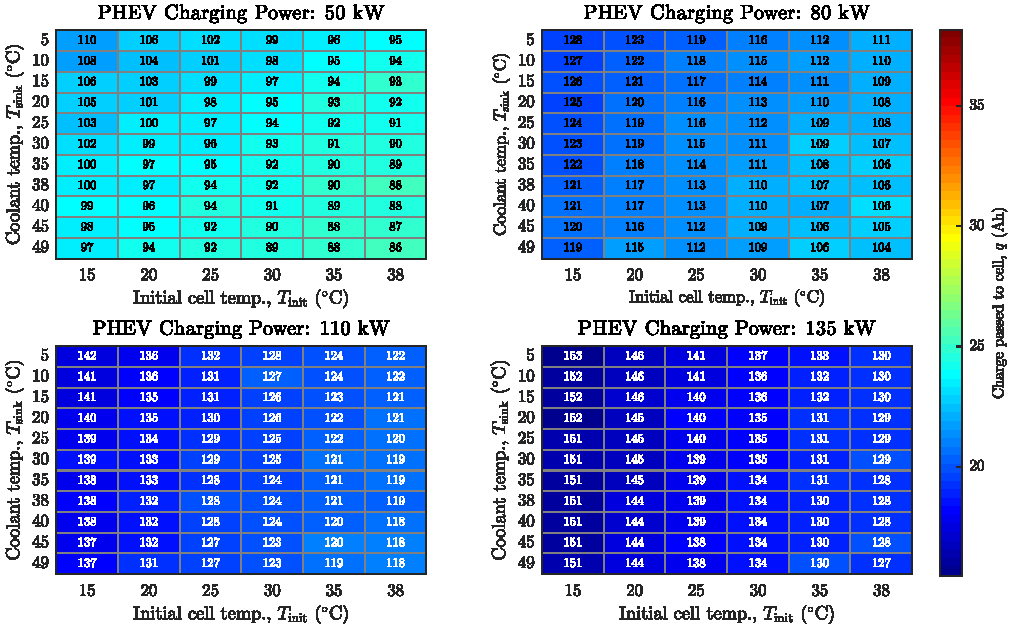
\includegraphics[width=\textwidth]{fig_generate_heatmap_PHEV}
        \caption[Optimal cell layer configurations for the \gls{phev}, presented for a range of
        fast charging powers and thermal conditions]{Optimal cell layer configurations for the \gls{phev}, presented for a range of
        fast charging powers and thermal conditions\footnotemark.}
        \label{fig:fig_generate_heatmap_PHEV}
        \mpfootnotes[1]
        \footnote{This figure was created by \mbox{Ian Campbell} who asserts copyright,
            with intellectual contributions from and the right to use asserted by
        \mbox{Krishnakumar Gopalakrishnan}.}
    \end{minipage}
\end{figure}


% satisfying specific acceleration and fast charging targets.
% that could potentially facilitate immediate adoption by
% industry.

% The proposed methodology accounts for the critical need to avoid lithium
% plating during fast charging and searches for the optimal layer configuration
% considering a range of thermal conditions. A numerical implementation of a cell
% model using a hybrid finite volume-spectral scheme is presented, wherein the
% model equations are suitably reformulated to directly accept power inputs,
% facilitating rapid and accurate searching of the layer design space. We show how
% thermal management design can limit vehicle driving range at high charging
% temperatures. We highlight how electrode materials exhibiting increased solid
% phase diffusion rates are as equally important for extended range as developing
% new materials with higher inherent capacity. We illustrate for a plug-in hybrid
% vehicle, how the proposed methodology facilitates common module design of
% battery packs, thereby reducing the cost of derivative vehicle models. To
% facilitate model based layer optimisation, we provide the open-source toolbox,
% BOLD (Battery Optimal Layer Design).

% Explain the goal of this chapter, to arrive at the number
% of layers to meet a given energy and power demand. The outcome is that a ready
% to use tool is made available to validate empirical layer choices. Special
% emphasis is placed on the \emph{methodology} since the results per se do not
% stand alone outside of the modelling regimen (universe we created). However, the
% value is on the methodology and its implementation in a toolbox which is
% immediately available for download and use by industry to confirm their
% empirical layer designs.


%%In the absence of access to cell manufacturing facilities to confirm and test the layer
%% Immediate adoption in industry.

\glsreset{xeV}
